\chapter{Learning-Based Validation of the Shared Representation}\label{sec:eval}

Chapter~\ref{sec:dataset} defined a shared route-aware graph representation for two construction paths: controlled SUMO simulation and conversion of repaired GPS trajectories. This chapter validates that representation from the learning side. The claim is intentionally practical: the same ETA learning pipeline can consume both exported dataset types, train successfully, and converge to useful held-out error levels. The model is used here as a downstream validator of the data contract, not as the main contribution of the report.

\section{Validation question}
The dataset layer is only useful if it supports a model-facing task without path-specific adapters. Therefore, the validation question is:
\begin{quote}
Can one route-aware ETA model be trained on graph bundles produced by both the simulation path and the trajectory-conversion path?
\end{quote}

The answer is evaluated on two representative bundles from the open-source workflow. The first comes from the three-zone simulation example, where traffic is controlled and sampled densely. The second comes from the Porto trajectory-conversion example, where sparse GPS traces are repaired, map matched, and projected into the same graph schema. Successful training on both sources shows that Chapter~\ref{sec:dataset}'s representation is not merely syntactically consistent; it is also learnable by a downstream ETA predictor.

\section{Representative bundles}
\begin{sloppypar}
Table~\ref{tab:dataset_stats_ch5} summarizes the two dataset instances used for learning validation. The simulation-backed bundle spans four weeks with dense 30\,s sampling. The trajectory-conversion bundle spans one year of Porto taxi data~\cite{porto2015pkdd}; its graph snapshots are trace-driven emitted steps, not a dense 30\,s grid over the full year. The two bundles therefore differ in scale, geography, and observability, while preserving the same node/edge feature interface.
\end{sloppypar}

\begin{table}[!htbp]
\caption[Representative dataset bundles from the open-source examples.]{Representative bundles from the open-source examples. Junction and road-edge counts are taken from SUMO \texttt{net.xml} files after excluding internal edges. Trip-rate, duration, and distance rows summarize the generated or converted trip populations used for the learning snapshot.}
\label{tab:dataset_stats_ch5}
\centering
\scriptsize
\setlength{\tabcolsep}{3pt}
\begin{tabular}{@{}lcc@{}}
\toprule
Quantity & Simulation & Trajectory conversion \\
\midrule
Temporal span & 4 weeks & 1 year \\
Project name & 3 zones city & Porto taxi \\
Trips after repair & 403\,848 & 1\,312\,637 \\
Trips per hour, avg.\ / std. & 601.0 / 366.4 & 149.8 / 128.7 \\
Trip duration (s), avg.\ / std. & 1\,011 / 416 & 1\,420 / 870 \\
Trip distance (km), avg.\ / std. & 13.07 / 6.42 & 18.40 / 11.20 \\
Junction nodes & 1\,031 & 75\,264 \\
Road edges (non-internal) & 1\,294 & 146\,816 \\
Approx.\ coverage area (km$^2$) & $\approx 203$ & $\approx 385$ \\
Graph snapshots (at $\Delta t$) & 80\,640 & 925\,644 \\
Snapshot period $\Delta t$ (s) & 30 & 30 \\
Node feat.\ dim.\ / edge feat.\ dim. & 28 / 6 & 28 / 6 \\
\bottomrule
\end{tabular}
\end{table}

\section{Model used for validation}
The predictor used in this report follows the DSTRA-GNN route-aware ETA model~\cite{dstra_gnn}. At a high level, it consumes a temporal window of graph snapshots, encodes the current traffic graph, incorporates each vehicle's remaining route context, and regresses ETA in seconds. This makes it suitable for validating the dataset representation because it relies on the same ingredients the representation is designed to expose: static road structure, dynamic vehicle state, road-level traffic signals, route suffixes, and time-aligned ETA labels.

The model itself is not the subject of this report. It is treated as a compatible downstream learner, and the full DSTRA-GNN paper is available with the supporting documents in the public repository \href{https://github.com/Turgibot/Multi-Variant-Simulated-Traffic-Dataset-Creator-and-Model-Tester/tree/master/docs}{docs folder}. The present work asks whether the dataset-creation workflow can feed such a learner from both construction paths.

As a sanity-check comparator, we also use a naive mean-duration baseline. For each dataset bundle, the baseline predicts the training-set average trip duration for every held-out journey. It has no access to route geometry, traffic state, graph context, or time-varying demand. Beating this baseline by a large margin indicates that the graph representation carries information beyond the marginal distribution of trip durations.

\section{Training protocol and metrics}
The simulation and trajectory-conversion bundles are trained separately with the same model interface and held-out evaluation protocol. Test journeys are disjoint from the trips used to fit the model for that bundle, and the mean-duration baseline uses only training-trip durations.

Performance is reported using five metrics: mean absolute error (MAE), root mean squared error (RMSE), mean absolute percentage error (MAPE), median absolute error (MedAE), and the 90th- and 95th-percentile absolute errors (P90, P95):
\[
\mathrm{MAE}=\frac{1}{N}\sum_{i=1}^{N}|\hat{y}_i-y_i|,
\quad
\mathrm{RMSE}=\sqrt{\frac{1}{N}\sum_{i=1}^{N}(\hat{y}_i-y_i)^2},
\]
\[
\mathrm{MAPE}(\%)=100\cdot\frac{1}{N}\sum_{i=1}^{N}\left|\frac{\hat{y}_i-y_i}{y_i}\right|,
\]
\[
\mathrm{MedAE}=\mathrm{median}\bigl(|\hat{y}_i-y_i|\bigr),
\quad
\mathrm{P}k = k\text{th percentile of }\bigl(|\hat{y}_i-y_i|\bigr).
\]
Here, $y_i$ is the realized remaining travel time and $\hat{y}_i$ is the prediction. MAE gives the typical absolute miss in seconds, RMSE penalizes large errors more strongly, and MAPE expresses error relative to trip duration. MedAE is robust to outliers and directly interpretable as the error that half of all predictions fall below. P90 and P95 quantify tail behavior: they state the absolute error that 90\% and 95\% of predictions, respectively, do not exceed. A known limitation of MAPE is that it becomes disproportionately large for very short trips, where even a small absolute error yields a high percentage; MedAE and P90/P95 are not affected by this distortion and therefore complement MAPE in characterizing short-trip performance.

\section{Training convergence}
Figure~\ref{fig:training_curves} illustrates typical validation behavior over the 100 epochs. The simulation curve descends faster because the simulation-backed bundle provides a denser sequence of active-traffic snapshots (roughly four times denser in this comparison), so dynamic vehicle and relation edges appear more frequently during training. This gives the model more repeated evidence about how traffic interactions affect ETA. The conversion curve reaches a comparable regime later because trajectory-derived snapshots are sparser and depend on repaired, segmented, and map-matched traces.

\begin{figure}[!htbp]
\centering
\resizebox{\linewidth}{!}{%
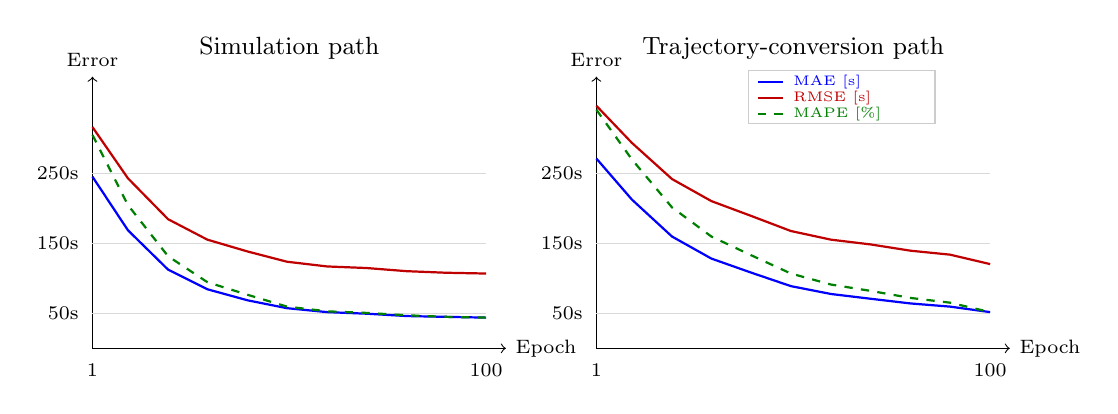
\begin{tikzpicture}

\begin{scope}[xshift=0cm]
  \draw[->] (0.8,0.7) -- (6.05,0.7) node[right] {\scriptsize Epoch};
  \draw[->] (0.8,0.7) -- (0.8,4.15) node[above] {\scriptsize Error};
  \draw[gray!30] (0.8,1.14) -- (5.8,1.14);
  \draw[gray!30] (0.8,2.03) -- (5.8,2.03);
  \draw[gray!30] (0.8,2.92) -- (5.8,2.92);
  \node[anchor=south] at (3.30,4.25) {\small Simulation path};
  \draw[blue, thick] (0.80,2.88) -- (1.25,2.20) -- (1.76,1.70) -- (2.26,1.45) -- (2.77,1.31) -- (3.27,1.21) -- (3.78,1.16) -- (4.28,1.14) -- (4.79,1.11) -- (5.29,1.10) -- (5.80,1.09);
  \draw[red!75!black, thick] (0.80,3.51) -- (1.25,2.86) -- (1.76,2.34) -- (2.26,2.08) -- (2.77,1.93) -- (3.27,1.80) -- (3.78,1.74) -- (4.28,1.72) -- (4.79,1.68) -- (5.29,1.66) -- (5.80,1.65);
  \draw[green!50!black, thick, dashed] (0.80,3.41) -- (1.25,2.52) -- (1.76,1.87) -- (2.26,1.54) -- (2.77,1.38) -- (3.27,1.23) -- (3.78,1.17) -- (4.28,1.15) -- (4.79,1.12) -- (5.29,1.10) -- (5.80,1.09);
  \node[anchor=north] at (0.8,0.62) {\scriptsize 1};
  \node[anchor=north] at (5.80,0.62) {\scriptsize 100};
  \node[anchor=east] at (0.75,1.14) {\scriptsize 50s};
  \node[anchor=east] at (0.75,2.03) {\scriptsize 150s};
  \node[anchor=east] at (0.75,2.92) {\scriptsize 250s};
\end{scope}


\begin{scope}[xshift=6.4cm]
  \draw[->] (0.8,0.7) -- (6.05,0.7) node[right] {\scriptsize Epoch};
  \draw[->] (0.8,0.7) -- (0.8,4.15) node[above] {\scriptsize Error};
  \draw[gray!30] (0.8,1.14) -- (5.8,1.14);
  \draw[gray!30] (0.8,2.03) -- (5.8,2.03);
  \draw[gray!30] (0.8,2.92) -- (5.8,2.92);
  \node[anchor=south] at (3.30,4.25) {\small Trajectory-conversion path};
  \draw[blue, thick] (0.80,3.11) -- (1.25,2.59) -- (1.76,2.12) -- (2.26,1.84) -- (2.77,1.66) -- (3.27,1.49) -- (3.78,1.39) -- (4.28,1.33) -- (4.79,1.27) -- (5.29,1.23) -- (5.80,1.16);
  \draw[red!75!black, thick] (0.80,3.78) -- (1.25,3.31) -- (1.76,2.85) -- (2.26,2.57) -- (2.77,2.38) -- (3.27,2.19) -- (3.78,2.08) -- (4.28,2.02) -- (4.79,1.94) -- (5.29,1.89) -- (5.80,1.77);
  \draw[green!50!black, thick, dashed] (0.80,3.73) -- (1.25,3.10) -- (1.76,2.49) -- (2.26,2.12) -- (2.77,1.88) -- (3.27,1.65) -- (3.78,1.51) -- (4.28,1.43) -- (4.79,1.34) -- (5.29,1.28) -- (5.80,1.16);
  \node[anchor=north] at (0.8,0.62) {\scriptsize 1};
  \node[anchor=north] at (5.80,0.62) {\scriptsize 100};
  \node[anchor=east] at (0.75,1.14) {\scriptsize 50s};
  \node[anchor=east] at (0.75,2.03) {\scriptsize 150s};
  \node[anchor=east] at (0.75,2.92) {\scriptsize 250s};
\end{scope}

\begin{scope}[shift={(9.25,3.65)}]
  \draw[fill=white, draw=gray!40] (-0.12,-0.10) rectangle (2.25,0.58);
  \draw[blue, thick] (0,0.43) -- (0.32,0.43) node[right] {\tiny MAE [s]};
  \draw[red!75!black, thick] (0,0.23) -- (0.32,0.23) node[right] {\tiny RMSE [s]};
  \draw[green!50!black, thick, dashed] (0,0.03) -- (0.32,0.03) node[right, align=left] {\tiny MAPE [\%]};
\end{scope}
\end{tikzpicture}
}
\caption[Representative 100-epoch validation curves for both construction paths.]{Representative 100-epoch validation curves for the two construction paths. Both curves converge, while the trajectory-conversion path converges later because its active-traffic snapshots are sparser; the denser simulation snapshots expose dynamic vehicle and relation edges more frequently during training.}
\label{fig:training_curves}
\end{figure}


Table~\ref{tab:learning_validation_results} reports the held-out metrics after 100 training epochs. The same route-aware model converges on both dataset sources. The trajectory-conversion result is slightly weaker, which is expected: converted GPS data is sparser, includes repaired segments, and depends on map matching before graph snapshots can be emitted. The MedAE values (29.8\,s for simulation, 34.7\,s for trajectory conversion) are considerably lower than the corresponding MAE values, confirming that the error distribution is right-skewed: the majority of journeys are predicted with a smaller absolute error than the mean suggests, while a tail of harder trips drives the average upward. The P90 and P95 columns quantify that tail: 90\% of simulation predictions fall within 103\,s and 90\% of trajectory-conversion predictions fall within 119\,s.

\begin{table}[!htbp]
\caption[Learning validation after 100 epochs: DSTRA vs.\ mean-duration baseline.]{Learning validation after 100 epochs: DSTRA vs.\ mean-duration baseline. MAE, RMSE, MedAE, P90, and P95 are in seconds; MAPE is in percent. MedAE is the median absolute error; P90/P95 are the 90th/95th percentile absolute errors.}
\label{tab:learning_validation_results}
\centering
\scriptsize
\setlength{\tabcolsep}{3pt}
\resizebox{\linewidth}{!}{%
\begin{tabular}{@{}l rrrrrr rrr@{}}
\toprule
 & \multicolumn{6}{c}{DSTRA} & \multicolumn{3}{c}{Mean baseline} \\
\cmidrule(lr){2-7}\cmidrule(lr){8-10}
Data source & MAE & RMSE & MAPE & MedAE & P90 & P95 & MAE & RMSE & MAPE \\
 & (s) & (s) & (\%) & (s) & (s) & (s) & (s) & (s) & (\%) \\
\midrule
Simulation           & 44.35 & 106.56 & 17.09 & 29.8 & 103 & 141 & 260.63 & 325.13 & 127.75 \\
Trajectory conversion & 51.69 & 120.56 & 20.08 & 34.7 & 119 & 163 & 282.66 & 352.41 & 138.50 \\
\bottomrule
\end{tabular}%
}
\end{table}

\begin{sloppypar}
The relative improvement over the naive baseline is large in both settings. On simulation-backed data, MAE drops from 260.63\,s to 44.35\,s, and the MedAE of 29.8\,s shows that the majority of journeys are predicted to within half a minute. On trajectory-converted data, MAE drops from 282.66\,s to 51.69\,s. This shows that the model is using route and traffic context exposed by the graph rather than simply learning an average journey duration.
\end{sloppypar}

\section{Interpretation}
The main conclusion is that both construction paths produce datasets that can train the same route-aware ETA model. This supports the central design of the project: simulation-derived and trajectory-derived traffic do not have to be identical, but they must be expressible through one model-facing representation.

This chapter therefore validates the representation as a learning artifact. Chapter~\ref{sec:web} continues the story from the application side: once a compatible model exists, the web environment can use it in an interactive route-selection and evaluation loop that records predictions against realized outcomes.

\FloatBarrier
